% "{'chapitre':'dyn_1d','classe':('PSI'),'type':('application'),'titre':'Réducteur','source':'C. Gamelon et P. Dubois','comp':('C1-05','C2-08','C2-09'),'corrige':False}"
%\setchapterimage{fig_00}
\chapter*{Application \arabic{cptApplication} \\ 
Réducteur -- \ifprof Corrigé \else Sujet \fi}

\addcontentsline{toc}{section}{Application \arabic{cptApplication} : Réducteur -- \ifprof Corrigé \else Sujet \fi}

\iflivret \stepcounter{cptApplication} \else
\ifprof  \stepcounter{cptApplication} \else \fi
\fi
\setcounter{question}{0}

\marginnote{D'après C. Gamelon \& P. Dubois.}
\marginnote{
\UPSTIcompetence[2]{C1-05}
\UPSTIcompetence[2]{C2-08}
\UPSTIcompetence[2]{C2-09}}

\begin{marginfigure}
\centering
%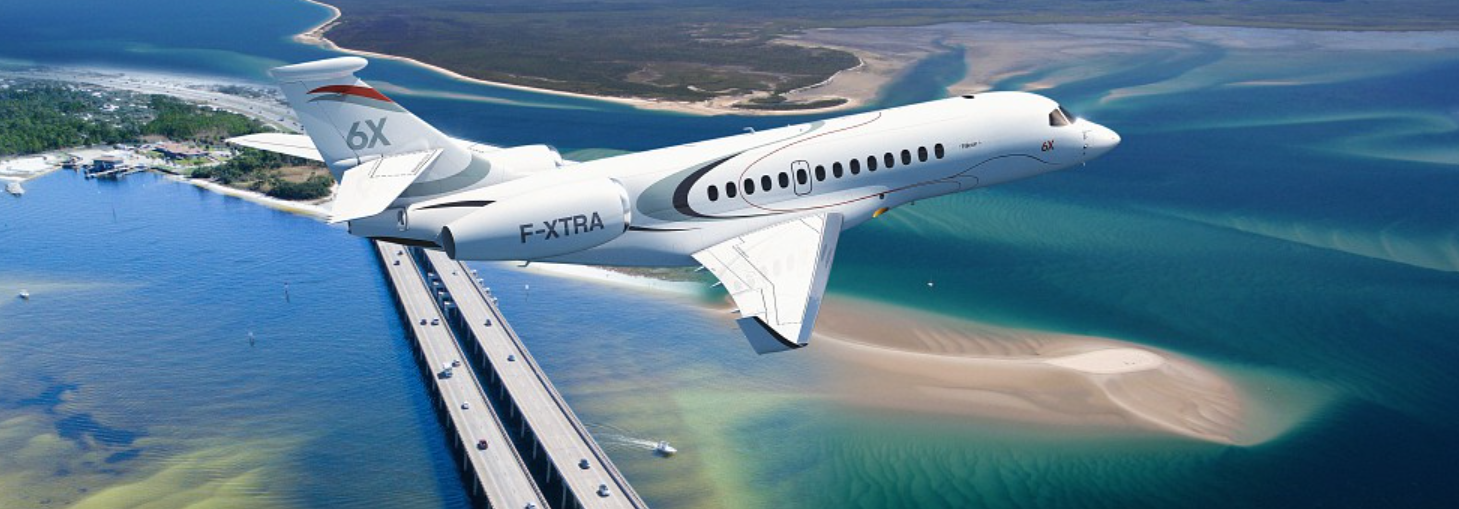
\includegraphics[width=\linewidth]{fig_00}
\end{marginfigure}


\section*{Exercice 1 -- Calcul de l'inertie équivalente d'un train simple}
\setcounter{subparagraph}{0}


\begin{marginfigure}
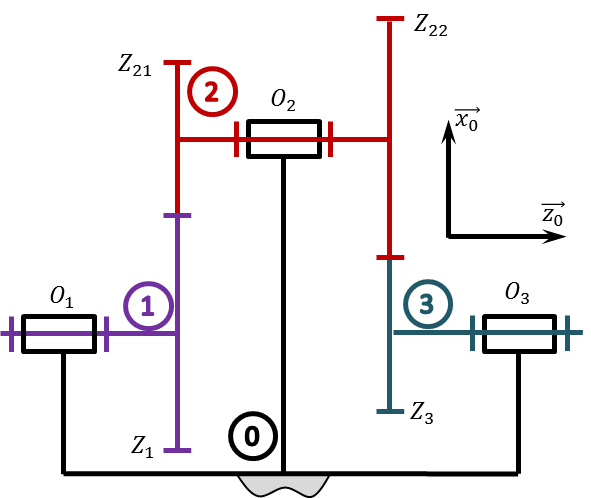
\includegraphics[width=\linewidth]{red_01}
\end{marginfigure}

On donne un train d'engrenages simple avec $Z_1$, $Z_{21}$, $Z_{23}$ et $Z_3$ le nombre de dents des roues dentées. On nomme $k_1$ le rapport du train de $S_1$ et $S_2$ avec $k_1=\dfrac{\omega(2/0)}{\omega(1/0)}$ et  
$k_2$ le rapport de $S_2$ et $S_3$ avec $k_2=\dfrac{\omega(3/0)}{\omega(2/0)}$. 

On applique en entrée, sur l'arbre 1, un couple moteur $C_m\vect{z_0}$ destiné à entraîner une charge, sur l'arbre 3, modélisée par un couple résistant  $C_r\vect{z_0}$



On rappelle que pour les engrenages à denture droite $d=mz$ avec $d$ le diamètre primitif, $m$ le module, $z$ le nombre de dents du pignon. $\omega(1/0)$, $\omega(2/0)$ et $\omega(3/0)$ sont les vitesses de rotation de $S_1$, $S_2$ et $S_3$ autour des axes $\left(O_1,\vect{x_g}\right)$, $\left(O_2,\vect{x_g}\right)$ et $\left(O_3,\vect{x_g}\right)$. Le repère galiléen $\mathcal{R}_g$ est lié au solide $S_0$. Les liaisons pivots sont supposées parfaites. Les moments d'inertie sont définies aux centres de masse $G_1=O_1$, $G_2=O_2$ et $G_3=O_3$ associées aux solides $S_1$, $S_2$ et $S_3$ suivant l'axe $\vect{z_0}$ sont de notés $J_1$, $J_2$ et $J_3$. 

Le train d'engrenage est entrainé par un couple moteur $C_m$ agissant sur la liaison pivot entre 1 et 0. 
Une poulie de rayon $R$ est placée sur l'extrémité droite de l'arbre 3. Une charge de masse $M$ y est suspendue. 

\question{Déterminer le rapport de réduction du train d'engrenages.}

\question{Déterminer l'inertie équivalente du réducteur seul ramené à l'axe moteur.}

\question{Déterminer l'inertie équivalente de l'ensemble réducteur et charge ramené à l'arbre moteur.}

\question{Déterminer la relation entre le couple d'entrée et le couple de sortie du réducteur.}

\question{Déterminer la relation entre le couple d'entrée, les grandeurs inertielles et l'accélération de l'arbre 1.}
